\chapter{Experiments}
\label{app:Experiments}

All experiments were ran on a virtual machine with four cores and 4GBs
or RAM. The virtual machines were hosted on the same computer and the
same programs were running during the experiments. Only one virtual
machine was tested at a time.

\section{Page Load Speed}
\label{sec:pageLoadSpeeds}

Each page of the website was loaded three times with an average being
given. Two results are recorded, one when the HTML file has finished
loading and another where the entire page is completely loaded.
A page is considered completely loaded when every requested
file is loaded and every request created via AJAX is complete. This
value is taken from the `Finish' value located at the bottom of
the Firefox developer console in the `Network' tab. These
experiments were done with caching turned off. Times were measured
in milliseconds. The experiments also started with a fresh website,
i.e. no users or messages. For redirects, the HTML values is recorded
for the page that started the redirect.

\begin{table}[H]
    \caption{Home Page load speed}
    \begin{center}
        \begin{tabular}{ | l | l | l | l | l |}
            \hline
            Run & Yesod HTML & Yesod Page & Django HTML & Django Page \\
            1 & 9 & 117 & 15 & 154 \\
            2 & 7 & 101 & 16 & 134 \\
            3 & 8 & 102 & 19 & 101 \\
            Average & 8 & 106.67 & 16.67 & 129.67 \\
            \hline
        \end{tabular}
    \end{center}
    \label{tab:pageLoadSpeeds}
\end{table}

\begin{table}[H]
    \caption{Search Page load speed}
    \begin{center}
        \begin{tabular}{ | l | l | l | l | l |}
            \hline
            Run & Yesod HTML & Yesod Page & Django HTML & Django Page \\
            1 & 4 & 155 & 15 & 120 \\
            2 & 4 & 120 & 14 & 115 \\
            3 & 5 & 136 & 18 & 107 \\
            Average & 4.33 & 137.33 & 15.67 & 114 \\
            \hline
        \end{tabular}
    \end{center}
    \label{tab:searchLoadSpeeds}
\end{table}

\begin{table}[H]
    \caption{Login Page load speed}
    \begin{center}
        \begin{tabular}{ | l | l | l | l | l |}
            \hline
            Run & Yesod HTML & Yesod Page & Django HTML & Django Page \\
            1 & 5 & 125 & 10 & 106 \\
            2 & 4 & 116 & 11 & 98 \\
            3 & 4 & 102 & 19 & 116 \\
            Average & 4.33 & 114.33 & 13.33 & 106.67 \\
            \hline
        \end{tabular}
    \end{center}
    \label{tab:loginLoadSpeeds}
\end{table}

\begin{table}[H]
    \caption{Signup Page load speed}
    \begin{center}
        \begin{tabular}{ | l | l | l | l | l |}
            \hline
            Run & Yesod HTML & Yesod Page & Django HTML & Django Page \\
            1 & 4 & 119 & 10 & 116 \\
            2 & 3 & 103 & 9 & 120 \\
            3 & 5 & 118 & 10 & 122 \\
            Average & 4 & 113.33 & 9.67 & 119.33 \\
            \hline
        \end{tabular}
    \end{center}
    \label{tab:signupLoadSpeeds}
\end{table}

\begin{table}[H]
    \caption{Create an account load speed}
    \begin{center}
        \begin{tabular}{ | l | l | l | l | l |}
            \hline
            Run & Yesod HTML & Yesod Page & Django HTML & Django Page \\
            1 & 398 & 554 & 85 & 218 \\
            2 & 364 & 585 & 82 & 248 \\
            3 & 360 & 547 & 82 & 243 \\
            Average & 374 & 562 & 83 & 236.33 \\
            \hline
        \end{tabular}
    \end{center}
    \label{tab:signupCreateLoadSpeeds}
\end{table}

\begin{table}[H]
    \caption{Log in to an account speed}
    \begin{center}
        \begin{tabular}{ | l | l | l | l | l |}
            \hline
            Run & Yesod HTML & Yesod Page & Django HTML & Django Page \\
            1 & 343 & 501 & 88 & 286 \\
            2 & 351 & 485 & 90 & 293 \\
            3 & 360 & 523 & 91 & 249 \\
            Average & 374 & 503 & 89.67 & 276 \\
            \hline
        \end{tabular}
    \end{center}
    \label{tab:loginLoginLoadSpeeds}
\end{table}

\begin{table}[H]
    \caption{Logout load speed speed}
    \begin{center}
        \begin{tabular}{ | l | l | l | l | l |}
            \hline
            Run & Yesod HTML & Yesod Page & Django HTML & Django Page \\
            1 & 1 & 220 & 15 & 314 \\
            2 & 1 & 160 & 14 & 303 \\
            3 & 1 & 193 & 15 & 321 \\
            Average & 1 & 191 & 14.67 & 312.67 \\
            \hline
        \end{tabular}
    \end{center}
    \label{tab:logoutLoadSpeeds}
\end{table}

\begin{table}[H]
    \caption{Current user's profile page}
    \begin{center}
        \begin{tabular}{ | l | l | l | l | l |}
            \hline
            Run & Yesod HTML & Yesod Page & Django HTML & Django Page \\
            1 & 9 & 373 & 20 & 351 \\
            2 & 12 & 351 & 20 & 446 \\
            3 & 9 & 312 & 31 & 383 \\
            Average & 10 & 345.33 & 23.67 & 393.33 \\
            \hline
        \end{tabular}
    \end{center}
    \label{tab:currentProfileLoadSpeeds}
\end{table}

\begin{table}[H]
    \caption{Creating message `test'}
    \begin{center}
        \begin{tabular}{ | l | l | l | l | l |}
            \hline
            Run & Yesod HTML & Yesod Page & Django HTML & Django Page \\
            1 & 11 & 481 & 13 & 433 \\
            2 & 14 & 412 & 18 & 413 \\
            3 & 14 & 385 & 17 & 384 \\
            Average & 13 & 426 & 16 & 410 \\
            \hline
        \end{tabular}
    \end{center}
    \label{tab:createMessageLoadSpeeds}
\end{table}

\begin{table}[H]
    \caption{Other profile page with three messages}
    \begin{center}
        \begin{tabular}{ | l | l | l | l | l |}
            \hline
            Run & Yesod HTML & Yesod Page & Django HTML & Django Page \\
            1 & 9 & 457 & 17 & 461 \\
            2 & 11 & 370 & 18 & 407 \\
            3 & 8 & 355 & 19 & 317 \\
            Average & 9.33 & 394 & 18 & 395 \\
            \hline
        \end{tabular}
    \end{center}
    \label{tab:otherProfileLoadSpeeds}
\end{table}

\begin{table}[H]
    \caption{Search for message `test', three results}
    \begin{center}
        \begin{tabular}{ | l | l | l | l | l |}
            \hline
            Run & Yesod HTML & Yesod Page & Django HTML & Django Page \\
            1 & 7 & 106 & 28 & 121 \\
            2 & 8 & 93 & 26 & 136 \\
            3 & 7 & 117 & 28 & 114 \\
            Average & 7.33 &  105.33 & 27.33 & 123.67 \\
            \hline
        \end{tabular}
    \end{center}
    \label{tab:searchMessageLoadSpeeds}
\end{table}

\begin{table}[H]
    \caption{Search for user `test', three results}
    \begin{center}
        \begin{tabular}{ | l | l | l | l | l |}
            \hline
            Run & Yesod HTML & Yesod Page & Django HTML & Django Page \\
            1 & 6 & 140 & 23 & 126 \\
            2 & 6 & 108 & 29 & 119 \\
            3 & 6 & 134 & 23 & 118 \\
            Average & 7.33 & 127.33 & 25 & 121 \\
            \hline
        \end{tabular}
    \end{center}
    \label{tab:searchUserLoadSpeeds}
\end{table}

\section{Resource Usage}

When yesod is running on the virtual machine, it uses around 239M of
memory according to htop. Django uses around 47M.

\begin{figure}[H]
    \centering
    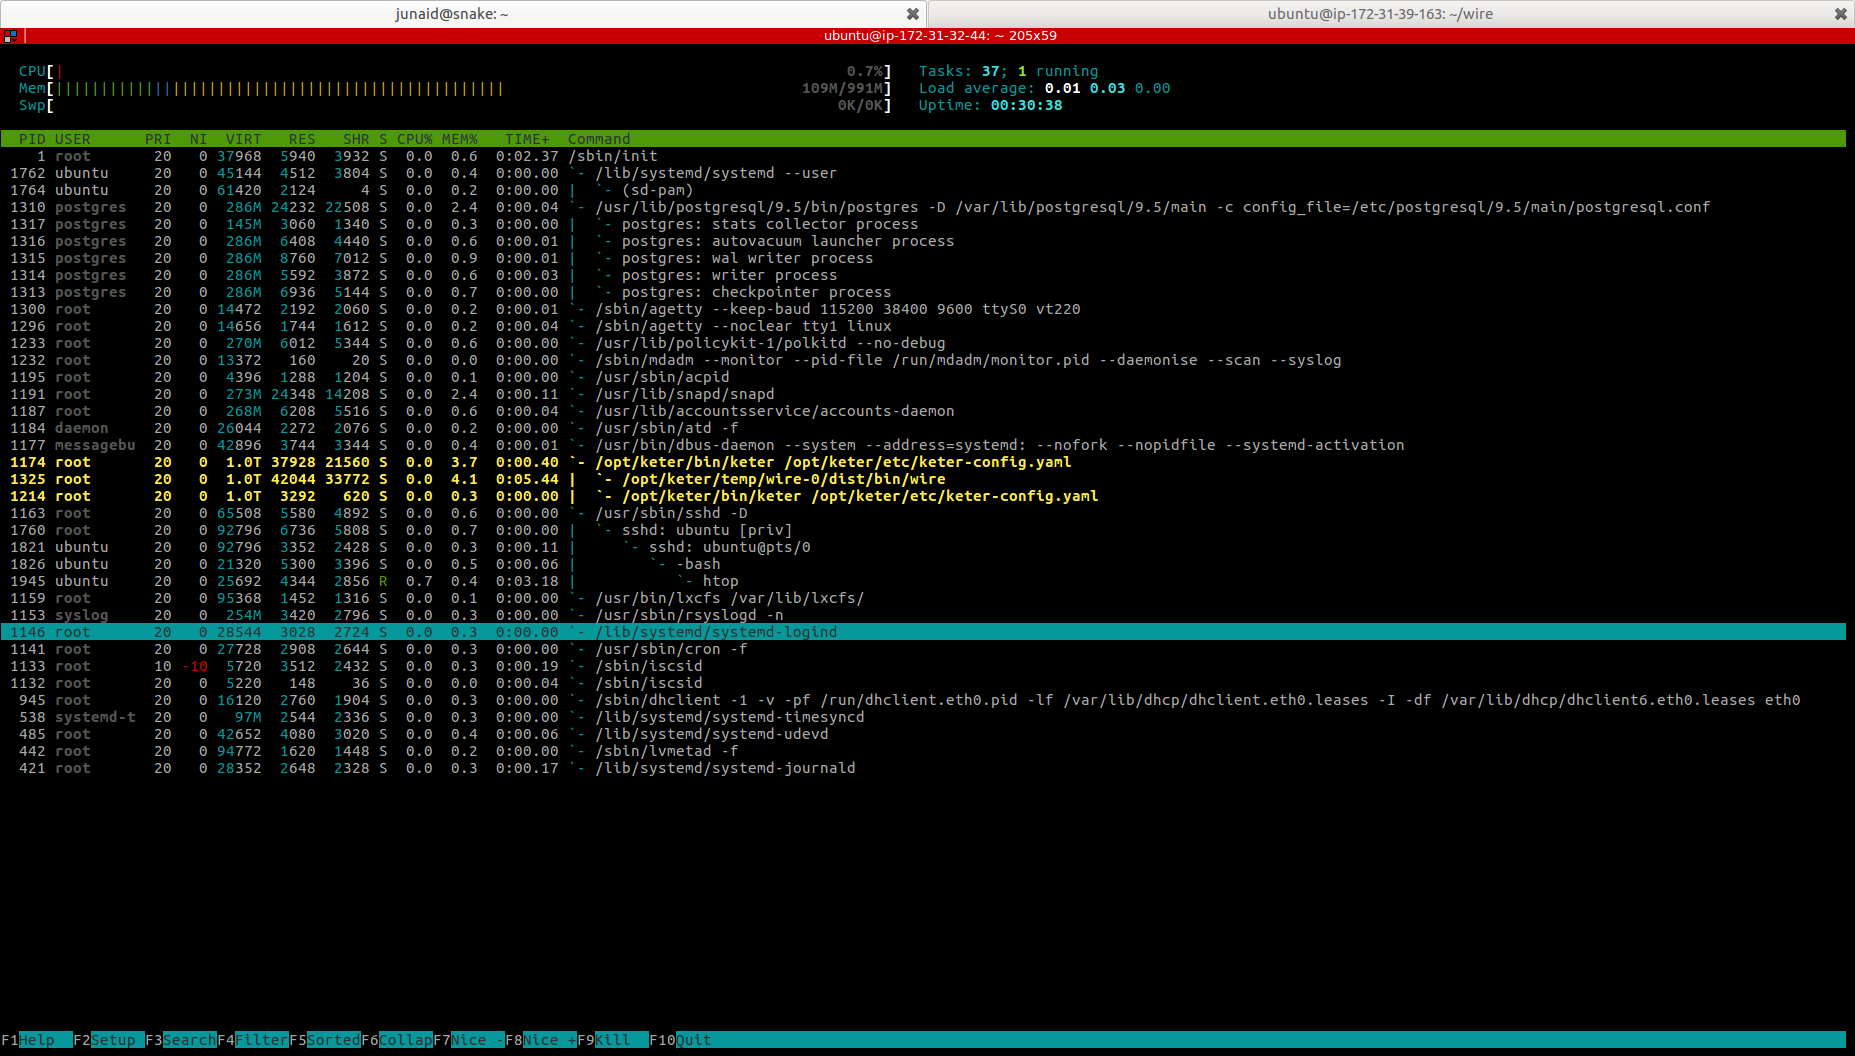
\includegraphics[width=0.7\textwidth]{final_report/pics/yesodIdle.png}
    \caption{Yesod htop output}
    \label{fig:yesodHtop}
\end{figure}

\begin{figure}[H]
    \centering
    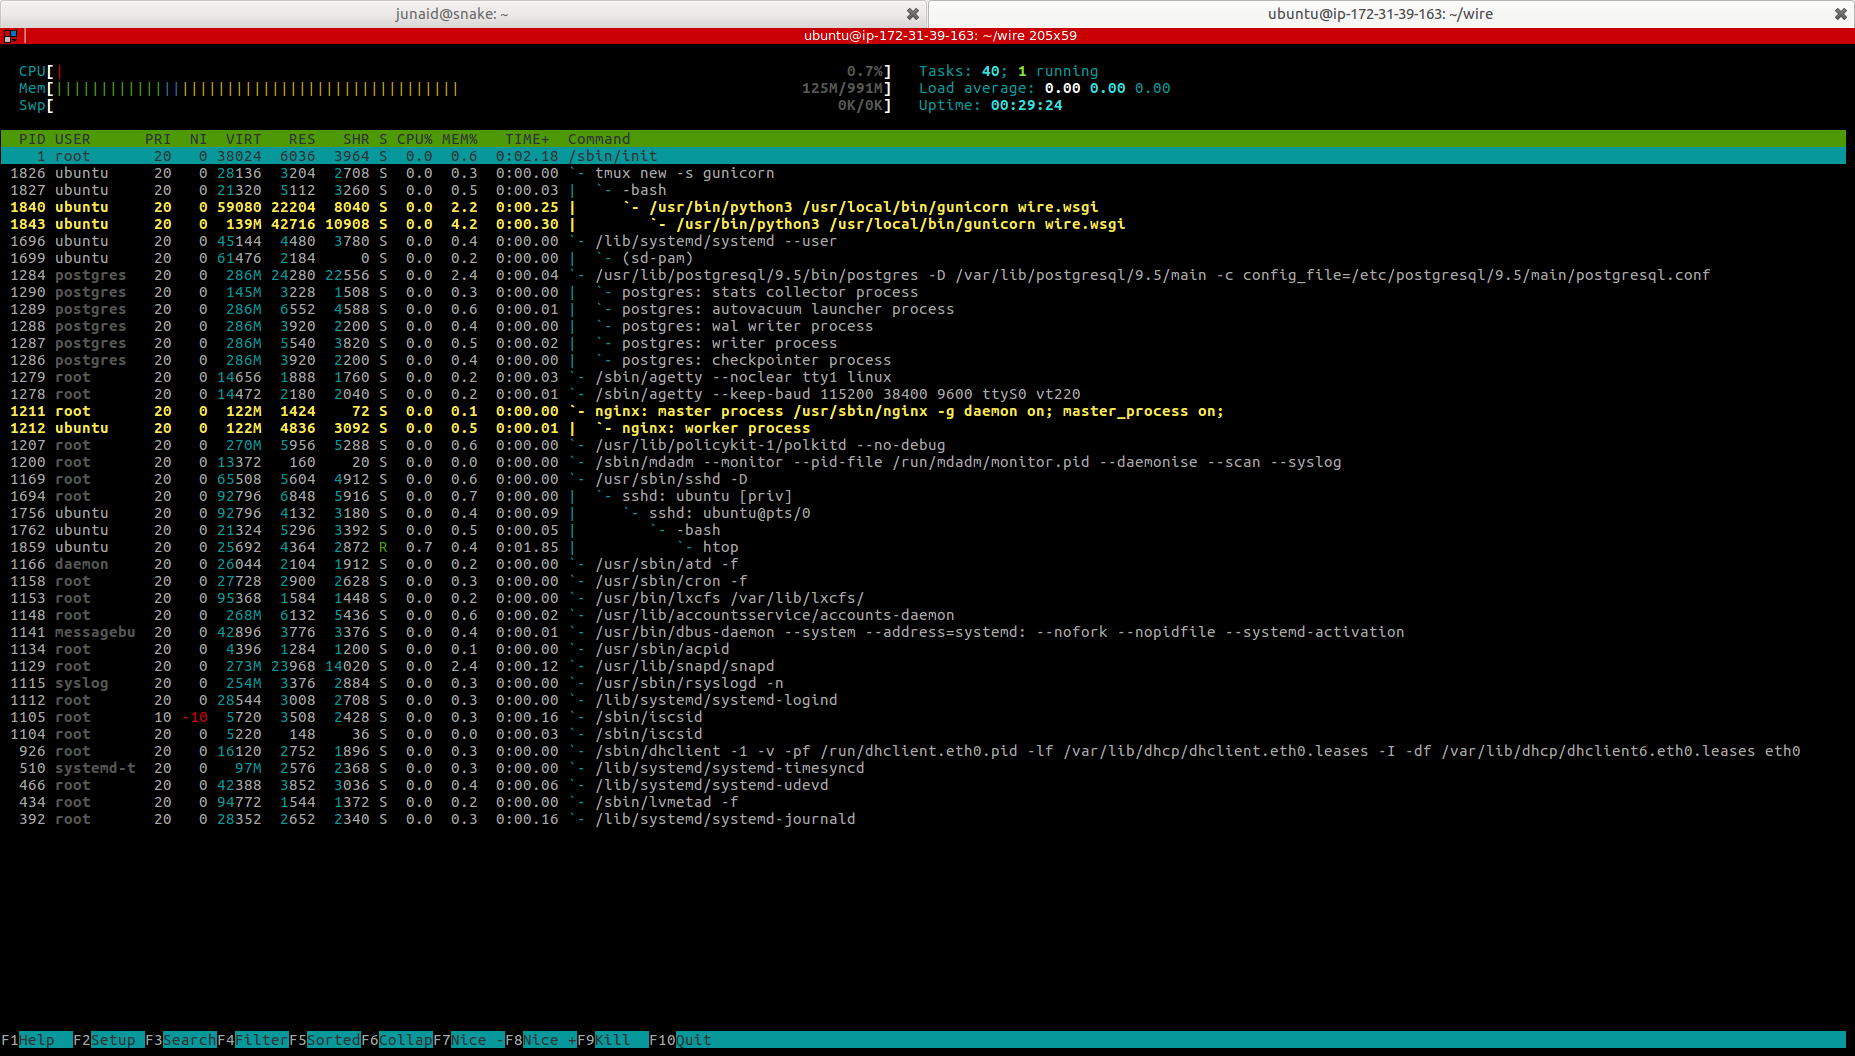
\includegraphics[width=0.7\textwidth]{final_report/pics/djangoIdle.png}
    \caption{Django htop output}
    \label{fig:djangoHtop}
\end{figure}

\section{Continuous Integration Build Times}

Both frameworks are stored on a git repository on GitHub. Whenever there is a
new commit, Travis CI, a continuous integration tools, starts to build
both frameworks and run tests. The tool will tell you whether or not tests
have passed. Django builds take around 2.5 minutes. Yesod builds take around
3.5-4 minutes. It should be noted that the first Yesod build took 32 minutes.
This was because the first build had to compile all the library files in the
Yesod project. Once these are compiled, they are cached, allowing them to
be used for future builds.

\begin{figure}[H]
    \centering
    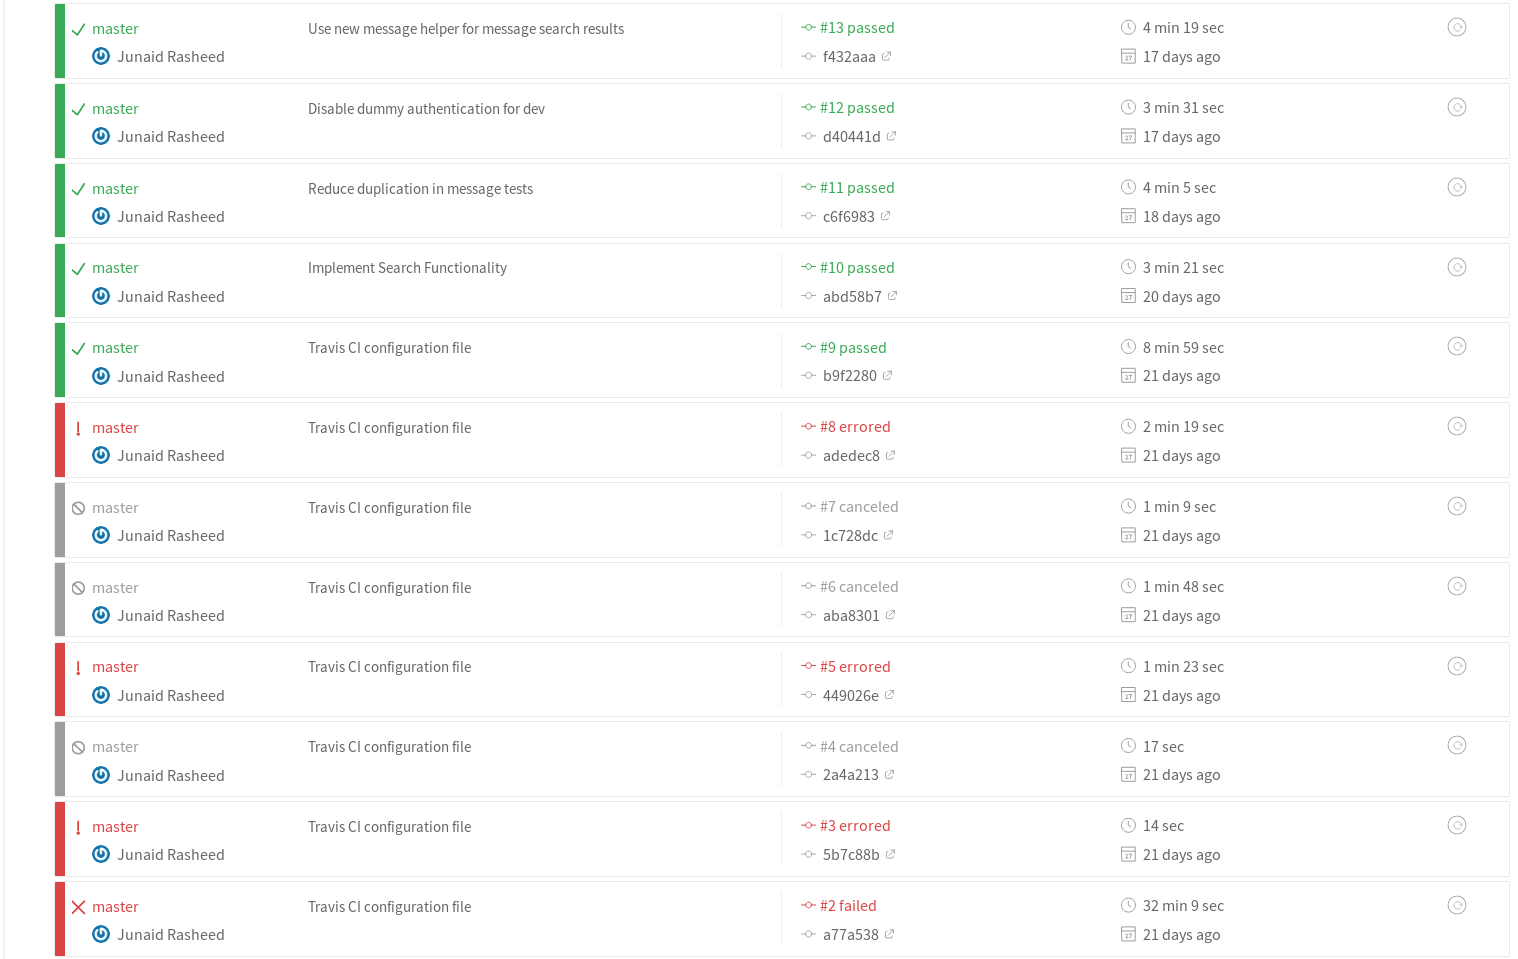
\includegraphics[width=0.7\textwidth]{final_report/pics/yesodTravis.png}
    \caption{Yesod Travis build times}
    \label{fig:yesodTravis}
\end{figure}

\begin{figure}[H]
    \centering
    
\includegraphics[width=0.7\textwidth]{final_report/pics/djangoTravis.png}
    \caption{Django Travis build times}
    \label{fig:djangoTravis}
\end{figure}

